%% -*- eval: (flyspell-mode 1); -*-

\chapter{Extraction et formalisation du parallélisme}

Le parallélisme dans un programme informatique est difficile à trouver automatiquement et la plupart du temps il est exprimé explicitement par le développeur. Il est alors nécessaire de lui offrir des outils permettant d'écrire le code parallèle simplement, en lui proposant notamment des fonctions et des mots-clés dans le langage choisi qui sont en accord à la fois avec les besoins matériels et à la fois avec les besoins algorithmiques. Ce chapitre dresse d'abord un état de l'art des principales solutions existantes, puis introduit les principaux objectifs du DSEL développé pendant le stage.

\section{Contexte}

Les applications parallèles sont utilisées depuis un certain nombres d'années afin d'obtenir des performances (en matière de rapidité, et en matière de taille du problème traité). Or il est difficile d'écrire des codes parallèles, ce qui a été évoqué au chapitre précédent. À ce titre divers outils pour faciliter la parallélisation sont apparus, tels que \textsf{ParaScope} dès $1989$ \cite{Art24} qui est éditeur de code interactif. Ces outils se décomposent en de nombreuses catégories à la fois par rapport aux utilisateurs qu'ils visent, et à la fois par rapport au parallélisme qu'ils permettent. Le cas d'application des stencils -- qui est le cas d'application du stage -- est alors explicité afin de voir comment interviennent les différents niveaux de parallélisme. 

\subsection{Expression du parallélisme}

Décrire les problèmes à résoudre et le parallélisme qu'ils peuvent utiliser peut se faire de différentes manières avec les moyens actuels. Notamment il est possible de regrouper quatre catégories qui sont les langages dédiés aux scientifiques (non spécialistes du HPC), les langages et compilateurs pour les développeurs de métier (mais non obligatoirement spécialistes du HPC), l'ensemble des bibliothèques et supports d'exécution spécialisés (destinés aux spécialistes du HPC), et en enfin les outils de formalisation des algorithmes employés (destinés aux spécialistes du HPC).

\paragraph{Langages dédiés aux scientifiques.}
Les langages dédiés aux scientifiques sont la plupart du temps des outils de simulation à destination d'experts dans ce domaine. Dans le cas des mathématiques par exemple, de nombreux logiciels définissant leur propre langage existent : \textsf{\href{http://www.wolfram.com/mathematica/}{Mathematica}}, \textsf{\href{http://fr.mathworks.com/}{MATLAB}} ou encore \textsf{\href{http://pari.math.u-bordeaux.fr/}{PARI/GP}} ; et une partie de leurs algorithmes sont parallélisés (au moins au niveau d'un processeur) pour des raisons de performances. Des initiatives plus poussées du côté du parallélisme sont également présentes en recherche comme \textsf{QIRAL} \cite{Art13,Art14} qui à partir d'algorithmes décrits en \LaTeX permet de générer un code parallèle optimisé pour les processeurs des ordinateurs courants -- mais pas pour les supercalculateurs --, il se base pour cela sur le système de réécriture \textsf{Maude} \cite{Art12}. La logique est alors la suivante : offrir à l'utilisateur les mêmes fonctions qui sont connues dans son domaine, en cachant l'implantation et la parallélisation de ces fonctions (telles qu'un calcul de facteurs premiers par exemple).

\paragraph{Langages dédiés au parallélisme.}
Quant il s'agit de développeurs souhaitant écrire du code parallèle sans forcément connaître les subtilités des machines d'exécutions, différents langages spécifiques ont été créés. De manière générale il s'agit en fait d'un langage déjà connu (\textsf{Java} ou \textsf{C/C++}) auquel sont ajoutés quelques mots-clés ou éléments de syntaxes (souvent pour les tableaux notamment) ; \textsf{\href{http://chapel.cray.com/}{Chapel}}, \textsf{\href{https://www.cilkplus.org/}{Cilk}}, \textsf{\href{http://upc.lbl.gov/}{UPC}}, \textsf{Lime} \cite{Art8}, \textsf{\href{http://x10-lang.org/}{X10}} et le langage proposé dans\cite{Art10} rentrent dans cette catégorie. Alors que les trois premiers cités sont très proches des langages d'origines, les trois derniers sont plus éloignés et proposent des paradigmes différents (comme les Map/Reduce dans \textsf{Lime} ou les horloges dans \textsf{X10}). Avec ces langages viennent souvent les compilateurs associés, toutefois parfois il s'agit plus simplement de réécriture automatique de code (vers un langage déjà existant) comme proposé par \textsf{Par4All} \cite{Ths2}. \textsf{Par4All} peut d'ailleurs être considéré comme un éditeur de code dédié au parallélisme, de même que le projet \textsf{Eclipse \href{http://www.eclipse.org/ptp/}{PTP}} (Parallel Tools Platform)ou les projets présentés dans les articles \cite{Art23,Art25}. Ces éditeurs rassemblent alors généralement plusieurs outils, et sont plus interactifs, mais leur parallélisation n'est pas toujours optimale.

\paragraph{Bibliothèques spécialisées.}
Pour atteindre un parallélisme optimal il est souvent nécessaire de descendre à un niveau plus proche du matériel. Plutôt que d'introduire quelques mots-clés supplémentaires, il s'agit alors de plusieurs dizaines de fonctions regroupées dans des bibliothèques. Il faut alors parfois utiliser différentes bibliothèques afin de gérer les différents niveaux de parallélisme (notamment interprocesseur et intraprocesseur). La bibliothèque utilisée dans le cadre du stage en fait partie : \textsf{\href{https://www.khronos.org/sycl}{SYCL}}. C'est celle qui est la plus haut niveau tout en offrant le plus de possibilités. La bibliothèque connue qui s'en rapproche le plus est \textsf{\href{https://www.khronos.org/opencl/}{OpenCL}} mais nécessite déjà plus d'efforts notamment pour gérer les communications entre les processeurs. En revanche \textsf{\href{http://openmp.org/wp/}{OpenMP}} (qui est en fait intégrée dans la plupart des compilateurs pour \textsf{Fortran}, \textsf{C/C++}) est beaucoup plus simple mais ne s'utilise que pour les processeurs génériques et non les processeurs graphiques. D'autres bibliothèques sont justement dédiés à la gestion de plusieurs types de processeurs en même temps, il s'agit des \emph{supports d'exécutions} tels que \textsf{\href{http://starpu.gforge.inria.fr/}{StarPU}} ou \textsf{\href{http://icl.utk.edu/parsec/}{PaRSEC}}. Comme la plupart des problèmes parallélisés sont liés à l'utilisation de grand tableaux, \textsf{Kokkos} \cite{Web5} et \textsf{\href{http://hpc.pnl.gov/globalarrays/}{Global Arrays}} permettent de simplifier leur utilisation et répartition sur les différents processeurs, mais ils ne gèrent pas le lancement des calculs contrairement aux supports d'exécutions. Plus spécifiquement encore l'article \cite{Art2} propose une solution simplifiant l'utilisation des tableaux avec le parallélisme, au sein d'un processeur. Enfin certaines rares bibliothèques se penchent plutôt sur les caractéristiques des algorithmes utilisés comme \textsf{SkePU} \cite{MstThs1}, qui s'apparente à un moteur d'exécution et utilise la formalisation de squelettes algorithmiques.


\paragraph{Formalisation des algorithmes.}
La formalisation des algorithmes parallèles se fait à travers différents outils comme la représentation polyédrique, utilisée lorsqu'il s'agit de parcours de tableaux au sein de boucles affines. Cette représentation permet d'ailleurs de mieux classifier les algorithmes, notamment en squelettes comme dans \textsf{SkePU} et \textsf{Bones} \cite{Art4,Art3,Art9}. Ces squelettes permettent de définir le motif d'accès aux données des tableaux impliqués dans le calcul de façon précise et ainsi de l'optimiser. Un tel exemple de motif -- plutôt général -- est le paradigme de \emph{Map/Reduce} qui est proposé par \textsf{SkePU} (ainsi que par le langage dédié \textsf{Lime} cité plus-haut). Cependant tous les algorithmes ne décrivent pas un calcul : certains sont au contraire destinés à ordonnancer les calculs, c'est-à-dire les répartir sur les différents processeurs disponibles. Encore plutôt à l'état de concept, c'est dans ce but que sont utilisés les \emph{composants} permettant les prédictions (et optimisations) du temps d'exécution tels que dans l'article \cite{Art7}, ainsi que les \emph{conteneurs intelligents} pour la gestion des communications avec la mémoire (et aussi les prédictions de temps) dans \textsf{SkePU} \cite[p.~78]{Ths1}.

\subsection{Cas d'application: les stencils}
\label{sec:stencil_base}

De nombreux problèmes notamment physiques ou mathématiques utilisent un certain type de calculs sur des grilles d'éléments qui sont regroupés sous le nom de \emph{stencils}. Dans ces problèmes chaque élément au sein d'une grille est calculé en fonction des valeurs de ses voisins. En une dimension, il s'agirait par exemple d'un tableau dans lequel chaque élément reçoit la somme de son voisin de droite et de celui de gauche. La notion de stencil est générique pour toute dimension, pour tout nombre de voisins impliqués, ainsi que pour leur disposition. La figure \ref{fig:stencil_base} présente un exemple de stencil en deux dimensions où seuls les quatre voisins immédiats interviennent dans le calcul de chaque élément bleu de la grille. Comme cette forme de stencil nécessite l'utilisation de points dans les deux sens de chaque dimension, une partie des points ne peuvent pas être mis à jour. Cette zone est appelée la zone \emph{fantôme} puisque qu'aucun calcul n'est fait sur ses éléments mais est obligatoire car ses éléments sont utilisés pour le calcul des éléments internes à la grille. Cette zone fantôme est représentée avec des éléments rouges sur la figure \ref{fig:stencil_base}.

\begin{figure}[!bp]
\floatbox[{\capbeside\thisfloatsetup{capbesideposition={right,center},capbesidewidth=4cm}}]{figure}[\FBwidth]
{\caption{Exemple d'une grille en deux dimensions avec un stencil à 4 points.}\label{fig:stencil_base}}
{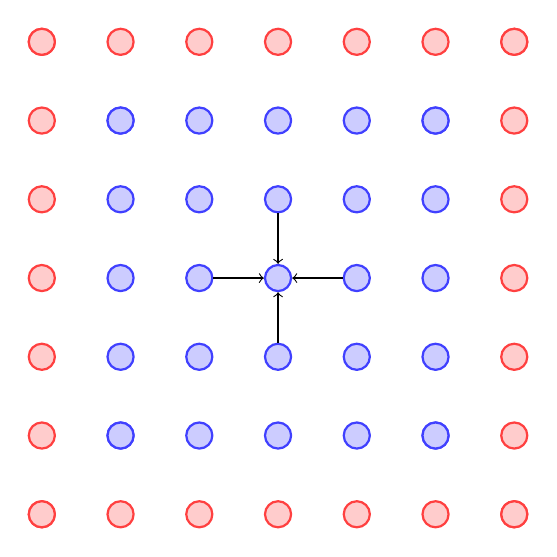
\begin{tikzpicture}
\tikzstyle{place}=[circle,thick,draw=blue!75,fill=blue!20,minimum size=2mm]

\node[place] (p1) at (0,0) {};
\node[place] (p2) at (0,1) {};
\node[place] (p3) at (1,0) {};
\node[place] (p4) at (-1,0) {};
\node[place] (p5) at (0,-1) {};

\node[place] () at (-1,-1) {};
\node[place] () at (-1,1) {};
\node[place] () at (1,-1) {};
\node[place] () at (1,1) {};

\foreach \x in {-2,...,2}
{
  \node[place] () at (\x,2) {};
  \node[place] () at (\x,-2) {};
  \node[place] () at (2,\x) {};
  \node[place] () at (-2,\x) {};
}

\draw[->] (p2) to (p1);
\draw[->] (p3) to (p1);
\draw[->] (p4) to (p1);
\draw[->] (p5) to (p1);

\tikzstyle{place}=[circle,thick,draw=red!75,fill=red!20,minimum size=2mm]

\foreach \x in {-3,...,3}
{
  \node[place] () at (\x,3) {};
  \node[place] () at (\x,-3) {};
  \node[place] () at (3,\x) {};
  \node[place] () at (-3,\x) {};
}



\end{tikzpicture}
}
\end{figure}

L'importante utilisation des stencils en recherche a conduit à des DSEL comme \textsf{Pochoir} \cite{Art18} ou  \textsf{Blitz++} \cite{Art5}, et des langages tels que \cite{Art19}, qui -- hormis \textsf{Blitz++} nécessitent leur propre compilateur afin d'effectuer des optimisations. Toutefois les stencils sont aussi utilisées dans des applications physiques non scientifiques, par exemple dans le calcul des graphismes de jeux vidéos \cite{Art15}. Dans les deux cas la performance est primordiale et il est donc nécessaire d'exploiter les possibilités de parallélisme des machines utilisées pour ces calculs.  

Si l'on suppose que la mise à jour de la grille par application du stencil n'est pas calculée en place -- c'est-à-dire que l'on dispose d'un tableau d'entrée dans lequel les éléments sont seulement lus, et d'un tableau de sortie où les résultats du calcul du stencil sur chaque élément sont stockés -- le stencil peut être appliqué à chaque élément bleu en même temps. Le parallélisme se trouve donc de manière très aisée dans ce type de problème. Avec une  machine possédant autant de cœurs que d'éléments dans la grille, la mise à jour de la grille se fait donc en une seule étape et tous les processeurs exécutent les mêmes instructions, simplement sur des éléments différents ; le calcul est donc bien adapté à une carte graphique qui regroupe justement ces caractéristiques : nombre élevé de cœurs et un même code s'exécutant sur tous ceux-ci. Puisque le calcul n'est pas en place, pour l'appliquer plusieurs fois d'affiliés il suffit d'intervertir les grilles d'entrées et de sortir entre chaque mise à jour, ou bien de recopier la sortie vers l'entrée, ce qui est toutefois plus lent.



Parler de la mémoire !


\section{Conception d'un DSEL pour les stencils}

A relire \cite{Art22}

\subsection{Objectifs sémantiques}

De quoi a-t-on besoin pour décrire un stencil

-> indices coefs

-> pattern du stencil

-> tableaux coefs

-> tableaux données

-> abstraire les structurations de données (copies tuiles, et data layout)

\subsection{Objectifs de performances}


-> tuiles/caches (data reuse)

-> calculs à la compilation


QCD \cite{Art1}
3.5D blocking \cite{Art11}

